\documentclass[compress,11pt]{beamer}

\usetheme{TALK}

\usepackage{minted}
\usemintedstyle{emacs}
\usepackage{graphbox}
% \usemintedstyle{colorful}
%\usemintedstyle{borland}
%\usemintedstyle{autumn}

\newminted{coq}{
frame=lines,
framesep=2mm,
fontsize=\scriptsize,
mathescape=true
}
\usepackage{commath}


% INFO DOCUMENT - TITRE, AUTEUR, INSTITUTION
\title{\bf\LARGE Enumerative Combinatorics in Coq/MathComp: \\
  Formal Power Series and the example of Catalan numbers}
\author{Florent Hivert}
\institute[LISN]{
  LISN / Université Paris Saclay / CNRS}
\date[December 2022]{Math Comp Workshop - December 2022}

\def\opstyle#1{\ensuremath{\operatorname{#1}}}

\newcommand{\free}[1]{\left\langle#1\right\rangle}
\newcommand{\N}{{\mathbb N}}
\newcommand{\Z}{{\mathbb Z}}
\newcommand{\C}{{\mathbb C}}
\newcommand{\Q}{{\mathbb Q}}
\newcommand{\SG}{{\mathfrak S}}

\newcommand{\qandq}{\text{\quad et\quad}}

\newcommand{\alphX}{{\mathbb X}}
\newcommand{\Count}{\opstyle{count}}
\newcommand{\List}{\opstyle{list}}
\newcommand{\Iter}{\opstyle{iter}}
\newcommand{\Unrank}{\opstyle{unrank}}
\newcommand{\Rank}{\opstyle{rank}}
\newcommand{\First}{\opstyle{first}}
\newcommand{\Next}{\opstyle{next}}
\newcommand{\Random}{\opstyle{random}}
\newcommand{\Oh}{O}

\newcommand{\card}{\opstyle{card}}
\newcommand{\Concat}{\opstyle{concat}}
\newcommand{\BS}{\opstyle{BitString}}
\newcommand{\Perm}{\opstyle{Perm}}
\newcommand{\BinTree}{\opstyle{BinTree}}
\newcommand{\Union}{\opstyle{Union}}
\newcommand{\Prod}{\opstyle{Prod}}
\newcommand{\Seq}{\opstyle{Seq}}
\newcommand{\PSet}{\opstyle{PSet}}
\newcommand{\MSet}{\opstyle{MSet}}
\newcommand{\Cycle}{\opstyle{Cycle}}

\newcommand{\mA}{\mathcal{A}}
\newcommand{\mB}{\mathcal{B}}
\newcommand{\mC}{\mathcal{C}}
\newcommand{\mD}{\mathcal{D}}
\newcommand{\mE}{\mathcal{E}}
\newcommand{\mI}{\mathcal{I}}
\newcommand{\mZ}{\mathcal{Z}}


%%%%%%%%%%%%%%%%%%%%% 
\renewcommand{\emph}[1]{{\color{red} #1}}
%------------------------------------------------------------------------------
\begin{document}

% PAGE D'ACCUEIL
\frame{\titlepage}

\begin{frame}{Outline}

  \begin{center}
    \url{https://github.com/hivert/FormalPowerSeries}
  \end{center}
  \tableofcontents
\end{frame}

\begin{frame}[fragile]
  % \includegraphics[trim=left bottom right top, clip]
  \parbox{4cm}{Flajolet-Sedgwick\\
    \textit{Analytic combinatorics}\\
    Figure I.2. \\
    The prehistory of Catalan numbers.
  }\quad
  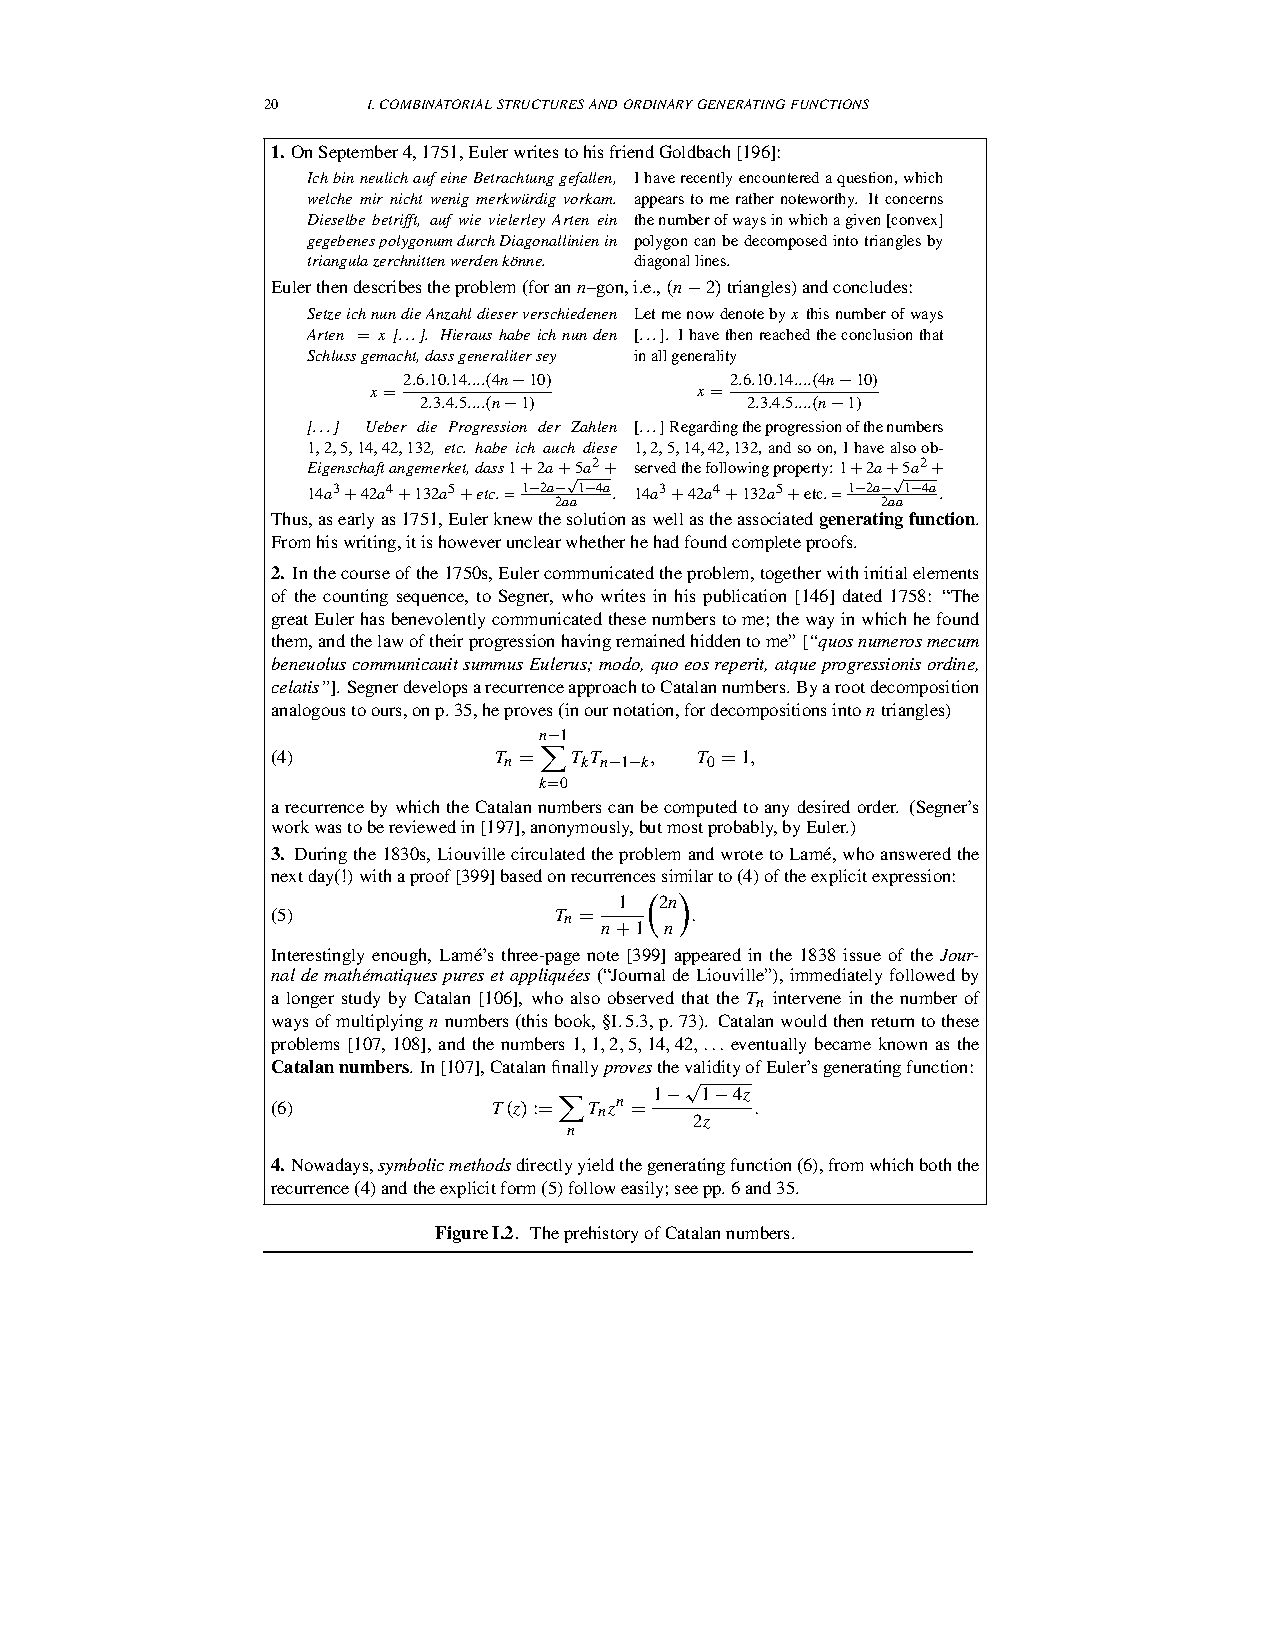
\includegraphics[align=c, trim=4.5cm 8.6cm 5cm 2.4cm, clip, width=6.2cm]{FlPage.pdf}
\end{frame}

\begin{frame}{Catalan numbers}

  \parbox{4cm}{
    \begin{center}
      Polygon triangulations\\[5mm]

      $1,1,2,5,14,42,132\dots$\\[3mm]
      $T_0=1$,\\[2mm]

      $\displaystyle T_n=\sum_{k=0}^{n-1}T_kT_{n-1-k}$\\[3mm]

      $\displaystyle T_n=\frac{1}{n+1}\binom{2n}{2}$
    \end{center}
  }\quad
  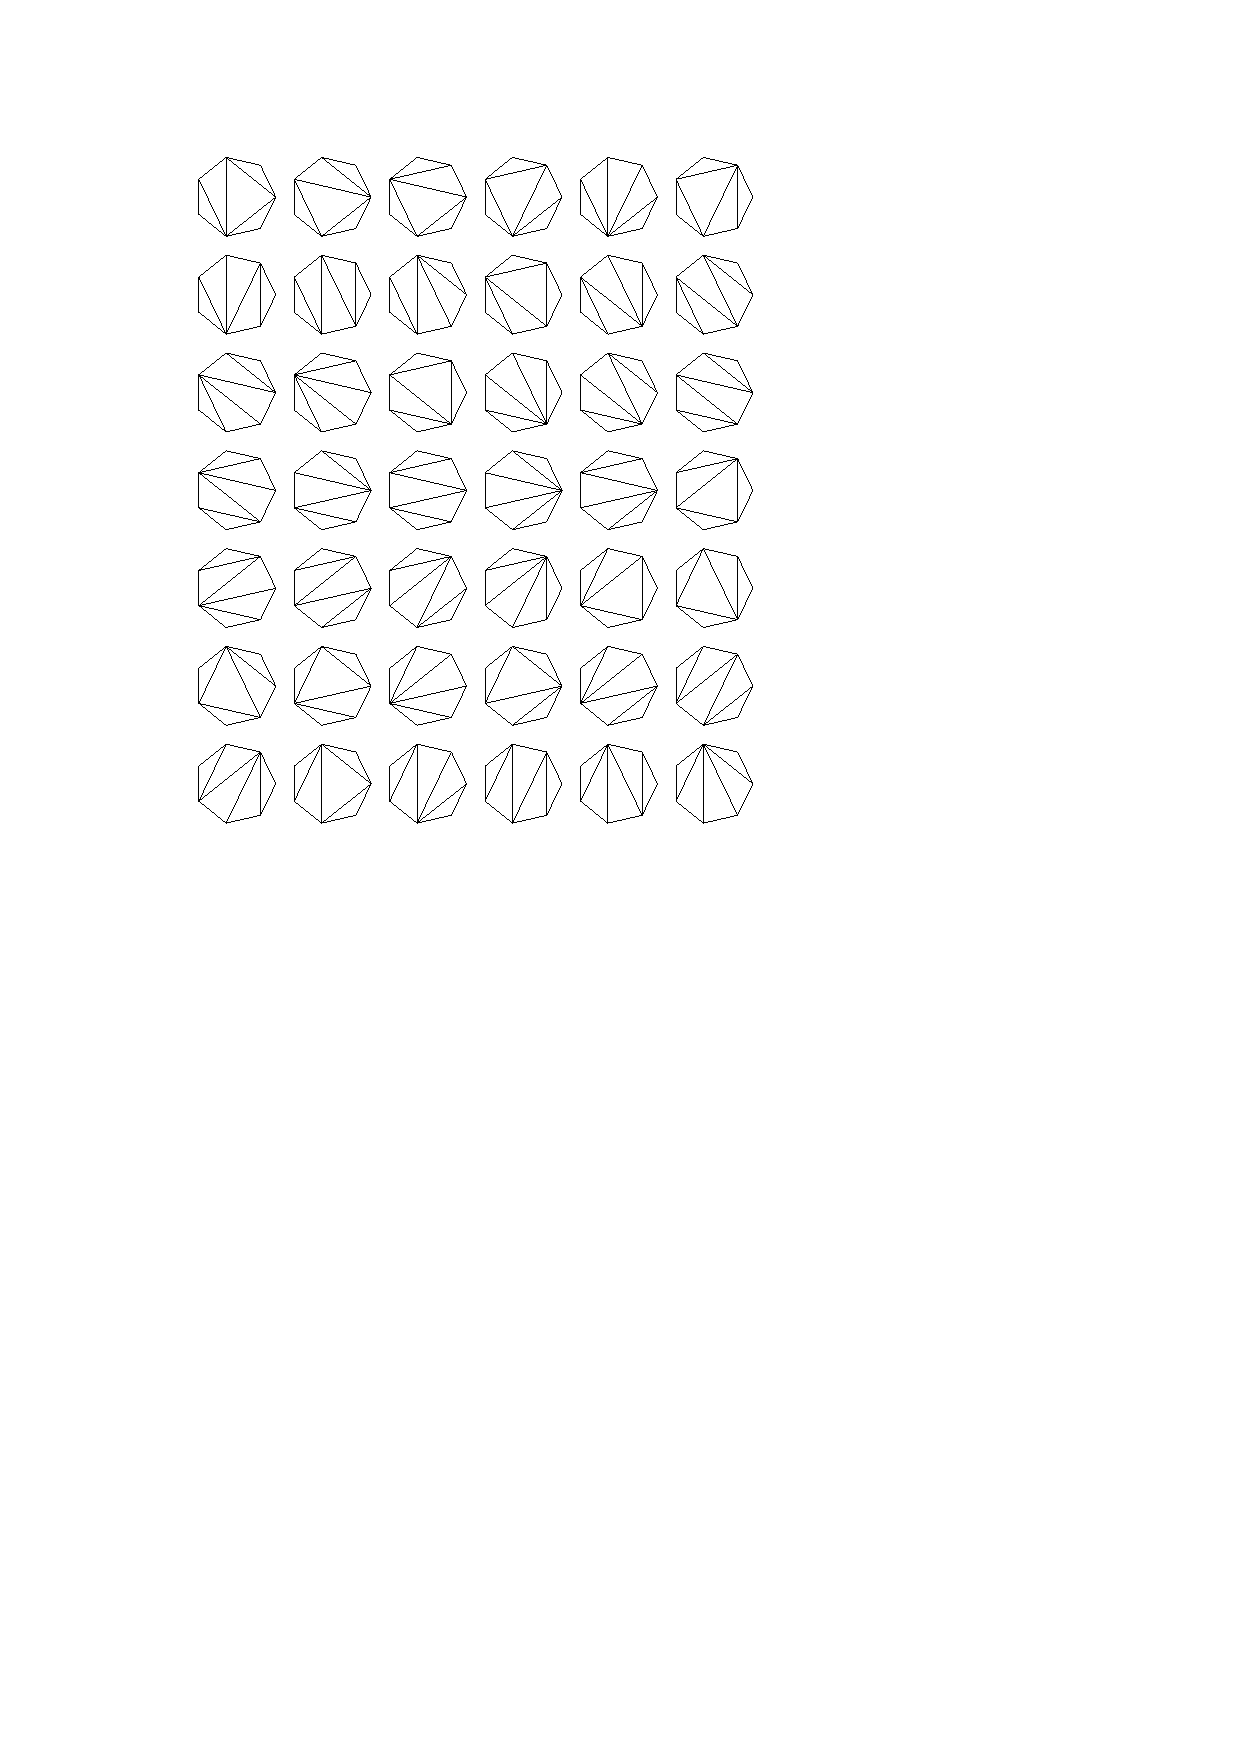
\includegraphics[align=c, trim=3cm 15cm 8cm 2.4cm, clip,
  width=6cm]{triangle.pdf}
\end{frame}

\begin{frame}{catalan}

  Euler, Segner, Liouville, Catalan, \dots
  \begin{equation*}
  \begin{split}
    T(z) &:= \sum_n T_n z^n = 1 + z +2 z^2 +5 z^3 + 14 z^4 + 42 z^5 + 132 z^6 +
    \dots \\
    &= \frac{1 - \sqrt{1-4z}}{2z}
  \end{split}
\end{equation*}
\end{frame}

\section{Enumerative Combinatorics}

\begin{frame}{Enumerative Combinatorics \\
    A short introduction from an algorithmic point of view}

  \Large
  \begin{tcolorbox}
    Counting and generating combinatorial objects
  \end{tcolorbox}
\end{frame}

\begin{frame}{Example of finite sets...}

  $n$-bits sequences:
  \begin{gather*}
    0\ 1 \\[4mm]
    00\ 01\ 10\ 11 \\[4mm]
    000\ 001\ 010\ 011\ 100\ 101\ 110\ 111 \\[4mm]
    0000\ 0001\ 0010\ 0011\ 0100\ 0101\ 0110\ 0111 \\
    1000\ 1001\ 1010\ 1011\ 1100\ 1101\ 1110\ 1111
  \end{gather*}
  Cardinality (number of elements): \url{https://oeis.org/A000079}
  \[2^n : 1, 2, 4, 8, 16, 32, 64, 128, 256, 512, 1024, 2048, 4096 \dots\]
\end{frame}


\begin{frame}{Permutation of $[1,2,\dots,n]$}
  % print(r"\ ".join("".join(str(i) for i in p) for p in Permutations(1).list()))
  \begin{gather*}
    1 \\[4mm]
    12\ 21 \\[4mm]
    123\ 132\ 213\ 231\ 312\ 321 \\[4mm]
    1234\ 1243\ 1324\ 1342\ 1423\ 1432\ 2134\ 2143\ 2314\ 2341\ 2413\ 2431\\
    3124\ 3142\ 3214\ 3241\ 3412\ 3421\ 4123\ 4132\ 4213\ 4231\ 4312\ 4321
  \end{gather*}
  Cardinality (number of elements): \url{https://oeis.org/A000142}
  \[n! : 1, 2, 6, 24, 120, 720, 5040, 40320, 362880, 3628800, 39916800 \dots\]
\end{frame}

\begin{frame}{Binary trees with $n$ nodes}

  {\newcommand{\nodea}{\node[draw,circle] (a) {$$};}
  \newcommand{\nodeb}{\node[draw,circle] (b) {$$};}
  \newcommand{\nodec}{\node[draw,circle] (c) {$$};}
  \newcommand{\noded}{\node[draw,circle] (c) {$$};}
  \tiny
  \begin{gather*}
    \begin{tikzpicture}
      \matrix[column sep=.1cm, row sep=.1cm,ampersand replacement=\&]{
        \nodea \\
      };
    \end{tikzpicture}\\[4mm]
    %%%%%
    \begin{tikzpicture}
      \matrix[column sep=.1cm, row sep=.1cm,ampersand replacement=\&]{
        \& \nodea  \&         \\
        \&         \& \nodeb  \\
      };
      \path[ultra thick] (a) edge (b);
    \end{tikzpicture}
    \begin{tikzpicture}
      \matrix[column sep=.1cm, row sep=.1cm,ampersand replacement=\&]{
        \& \nodea  \&         \\
        \nodeb  \&         \&         \\
      };
      \path[ultra thick] (a) edge (b);
    \end{tikzpicture}\\[4mm]
    %%%
    \begin{tikzpicture}
      \matrix[column sep=.1cm, row sep=.1cm,ampersand replacement=\&]{
        \& \nodea  \&         \&         \&         \\
        \&         \&         \& \nodeb  \&         \\
        \&         \&         \&         \& \nodec  \\
      };
      \path[ultra thick] (b) edge (c)
      (a) edge (b);
    \end{tikzpicture}
    \begin{tikzpicture}
      \matrix[column sep=.1cm, row sep=.1cm,ampersand replacement=\&]{
        \& \nodea  \&         \&         \&         \\
        \&         \&         \& \nodeb  \&         \\
        \&         \& \nodec  \&         \&         \\
      };
      \path[ultra thick] (b) edge (c)
      (a) edge (b);
    \end{tikzpicture}
    \begin{tikzpicture}
      \matrix[column sep=.1cm, row sep=.1cm,ampersand replacement=\&]{
        \& \nodea  \&         \\
        \nodeb  \&         \& \nodec  \\
      };
      \path[ultra thick] (a) edge (b) edge (c);
    \end{tikzpicture}
    \begin{tikzpicture}
      \matrix[column sep=.1cm, row sep=.1cm,ampersand replacement=\&]{
        \&         \&         \& \nodea  \&         \\
        \& \nodeb  \&         \&         \&         \\
        \&         \& \nodec  \&         \&         \\
      };
      \path[ultra thick] (b) edge (c)
      (a) edge (b);
    \end{tikzpicture}
    \begin{tikzpicture}
      \matrix[column sep=.1cm, row sep=.1cm,ampersand replacement=\&]{
        \&         \&         \& \nodea  \&         \\
        \& \nodeb  \&         \&         \&         \\
        \nodec  \&         \&         \&         \&         \\
      };
      \path[ultra thick] (b) edge (c)
      (a) edge (b);
    \end{tikzpicture}
  \end{gather*}}
\end{frame}


\begin{frame}{Binary trees with $n$ nodes}

  {\newcommand{\nodea}{\node[draw,circle] (a) {$$};}
  \newcommand{\nodeb}{\node[draw,circle] (b) {$$};}
  \newcommand{\nodec}{\node[draw,circle] (c) {$$};}
  \newcommand{\noded}{\node[draw,circle] (d) {$$};}
  \tiny
  \begin{gather*}
\begin{tikzpicture}
\matrix[column sep=.1cm, row sep=.1cm,ampersand replacement=\&]{
         \& \nodea  \&         \&         \&         \&         \&         \\
         \&         \&         \& \nodeb  \&         \&         \&         \\
         \&         \&         \&         \&         \& \nodec  \&         \\
         \&         \&         \&         \&         \&         \& \noded  \\
};
\path[ultra thick] (c) edge (d)
	(b) edge (c)
	(a) edge (b);
\end{tikzpicture}
\begin{tikzpicture}
\matrix[column sep=.1cm, row sep=.1cm,ampersand replacement=\&]{
         \& \nodea  \&         \&         \&         \&         \&         \\
         \&         \&         \& \nodeb  \&         \&         \&         \\
         \&         \&         \&         \&         \& \nodec  \&         \\
         \&         \&         \&         \& \noded  \&         \&         \\
};
\path[ultra thick] (c) edge (d)
	(b) edge (c)
	(a) edge (b);
\end{tikzpicture}
\begin{tikzpicture}
\matrix[column sep=.1cm, row sep=.1cm,ampersand replacement=\&]{
         \& \nodea  \&         \&         \&         \\
         \&         \&         \& \nodeb  \&         \\
         \&         \& \nodec  \&         \& \noded  \\
};
\path[ultra thick] (b) edge (c) edge (d)
	(a) edge (b);
\end{tikzpicture}
\begin{tikzpicture}
\matrix[column sep=.1cm, row sep=.1cm,ampersand replacement=\&]{
         \& \nodea  \&         \&         \&         \&         \&         \\
         \&         \&         \&         \&         \& \nodeb  \&         \\
         \&         \&         \& \nodec  \&         \&         \&         \\
         \&         \&         \&         \& \noded  \&         \&         \\
};
\path[ultra thick] (c) edge (d)
	(b) edge (c)
	(a) edge (b);
\end{tikzpicture}
\begin{tikzpicture}
\matrix[column sep=.1cm, row sep=.1cm,ampersand replacement=\&]{
         \& \nodea  \&         \&         \&         \&         \&         \\
         \&         \&         \&         \&         \& \nodeb  \&         \\
         \&         \&         \& \nodec  \&         \&         \&         \\
         \&         \& \noded  \&         \&         \&         \&         \\
};
\path[ultra thick] (c) edge (d)
	(b) edge (c)
	(a) edge (b);
\end{tikzpicture}\\
\begin{tikzpicture}
\matrix[column sep=.1cm, row sep=.1cm,ampersand replacement=\&]{
         \& \nodea  \&         \&         \&         \\
 \nodeb  \&         \&         \& \nodec  \&         \\
         \&         \&         \&         \& \noded  \\
};
\path[ultra thick] (c) edge (d)
	(a) edge (b) edge (c);
\end{tikzpicture}
\begin{tikzpicture}
\matrix[column sep=.1cm, row sep=.1cm,ampersand replacement=\&]{
         \& \nodea  \&         \&         \&         \\
 \nodeb  \&         \&         \& \nodec  \&         \\
         \&         \& \noded  \&         \&         \\
};
\path[ultra thick] (c) edge (d)
	(a) edge (b) edge (c);
\end{tikzpicture}
\begin{tikzpicture}
\matrix[column sep=.1cm, row sep=.1cm,ampersand replacement=\&]{
         \&         \&         \& \nodea  \&         \\
         \& \nodeb  \&         \&         \& \noded  \\
         \&         \& \nodec  \&         \&         \\
};
\path[ultra thick] (b) edge (c)
	(a) edge (b) edge (d);
\end{tikzpicture}
\begin{tikzpicture}
\matrix[column sep=.1cm, row sep=.1cm,ampersand replacement=\&]{
         \&         \&         \& \nodea  \&         \\
         \& \nodeb  \&         \&         \& \noded  \\
 \nodec  \&         \&         \&         \&         \\
};
\path[ultra thick] (b) edge (c)
	(a) edge (b) edge (d);
\end{tikzpicture}
\begin{tikzpicture}
\matrix[column sep=.1cm, row sep=.1cm,ampersand replacement=\&]{
         \&         \&         \&         \&         \& \nodea  \&         \\
         \& \nodeb  \&         \&         \&         \&         \&         \\
         \&         \&         \& \nodec  \&         \&         \&         \\
         \&         \&         \&         \& \noded  \&         \&         \\
};
\path[ultra thick] (c) edge (d)
	(b) edge (c)
	(a) edge (b);
\end{tikzpicture}\\
\begin{tikzpicture}
\matrix[column sep=.1cm, row sep=.1cm,ampersand replacement=\&]{
         \&         \&         \&         \&         \& \nodea  \&         \\
         \& \nodeb  \&         \&         \&         \&         \&         \\
         \&         \&         \& \nodec  \&         \&         \&         \\
         \&         \& \noded  \&         \&         \&         \&         \\
};
\path[ultra thick] (c) edge (d)
	(b) edge (c)
	(a) edge (b);
\end{tikzpicture}
\begin{tikzpicture}
\matrix[column sep=.1cm, row sep=.1cm,ampersand replacement=\&]{
         \&         \&         \& \nodea  \&         \\
         \& \nodeb  \&         \&         \&         \\
 \nodec  \&         \& \noded  \&         \&         \\
};
\path[ultra thick] (b) edge (c) edge (d)
	(a) edge (b);
\end{tikzpicture}
\begin{tikzpicture}
\matrix[column sep=.1cm, row sep=.1cm,ampersand replacement=\&]{
         \&         \&         \&         \&         \& \nodea  \&         \\
         \&         \&         \& \nodeb  \&         \&         \&         \\
         \& \nodec  \&         \&         \&         \&         \&         \\
         \&         \& \noded  \&         \&         \&         \&         \\
};
\path[ultra thick] (c) edge (d)
	(b) edge (c)
	(a) edge (b);
\end{tikzpicture}
\begin{tikzpicture}
\matrix[column sep=.1cm, row sep=.1cm,ampersand replacement=\&]{
         \&         \&         \&         \&         \& \nodea  \&         \\
         \&         \&         \& \nodeb  \&         \&         \&         \\
         \& \nodec  \&         \&         \&         \&         \&         \\
 \noded  \&         \&         \&         \&         \&         \&         \\
};
\path[ultra thick] (c) edge (d)
	(b) edge (c)
	(a) edge (b);
\end{tikzpicture}
\end{gather*}}
  Cardinality (number of elements): \url{https://oeis.org/A000142}
  \[\operatorname{Cat}(n) : 1, 2, 5, 14, 42, 132, 429, 1430, 4862,
  16796, 58786, 208012 \dots\]
\end{frame}

\begin{frame}{Unlabelled graphs with $n$ vertices}

  Unlabelled = upto isomorphism\bigskip

  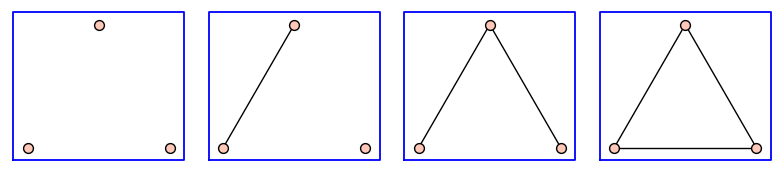
\includegraphics[width=5cm]{media/graphs-3.png}
\quad
  \raisebox{-1.3cm}{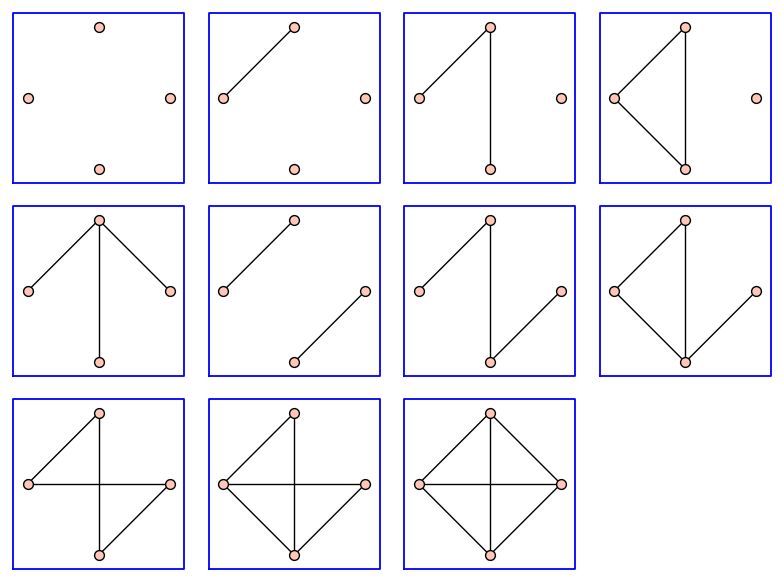
\includegraphics[width=5cm]{media/graphs-4.png}}
  \bigskip

  Cardinality (number of elements): \url{https://oeis.org/A000088}
  \[\operatorname{Gr}(n) :
  1, 2, 4, 11, 34, 156, 1044, 12346, 274668, 12005168, 1018997864
  \dots\]
\end{frame}

\begin{frame}{Unlabelled graphs with $5$ vertices:}

  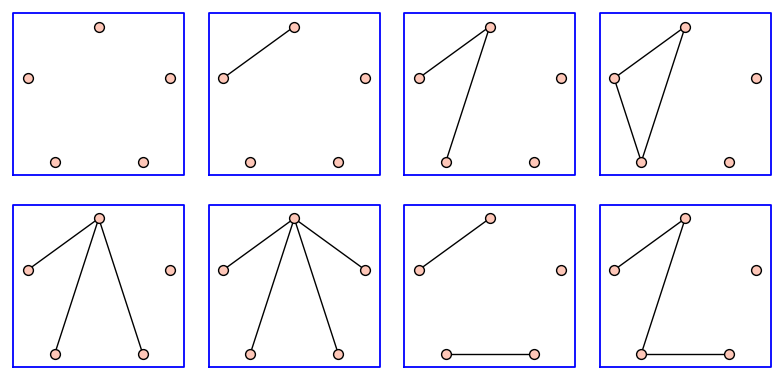
\includegraphics[width=5cm]{media/graphs-5-1.png}
  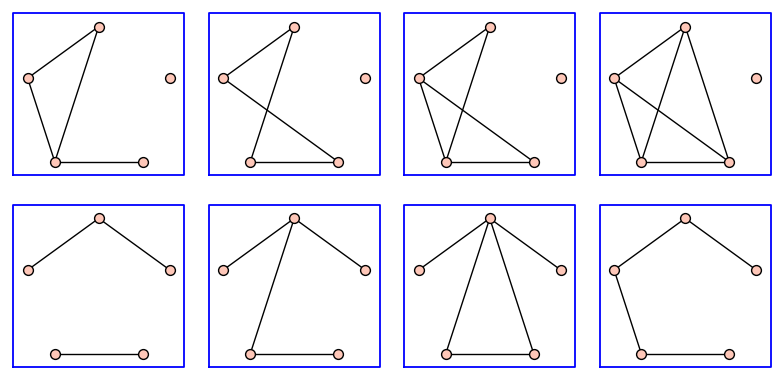
\includegraphics[width=5cm]{media/graphs-5-2.png}\\
  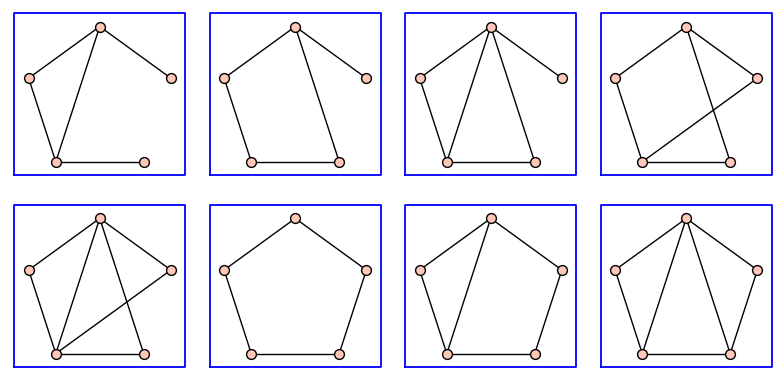
\includegraphics[width=5cm]{media/graphs-5-3.png}
  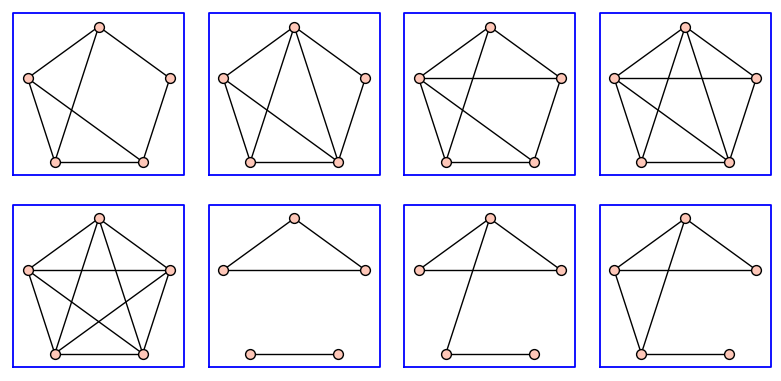
\includegraphics[width=5cm]{media/graphs-5-4.png}\\
  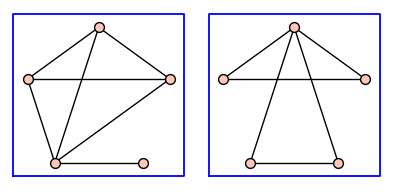
\includegraphics[width=2.5cm]{media/graphs-5-5.png}
\end{frame}


\begin{frame}{More «real life examples»}
  \begin{itemize}
  \item XML document with $n$ balises
    \bigskip

  \item $n$ character program in C
    \bigskip

  \item possible execution pathes in a code
  \end{itemize}
\end{frame}

\begin{frame}{Combinatorial Generation}

  \begin{QUESTION}
    \textbf{Find efficient algorithms}
    \begin{itemize}
    \item count, find the list, iterate
    \item fair random sampling
    \end{itemize}
  \end{QUESTION}
  Application:
  \begin{itemize}
  \item \textbf{search of a solution} using brute force or randomization
  \item analysis of algorithms, \textbf{complexity computation}
  \item \textbf{tests}, fuzzing
  \item biology, chemistry, statistical physics
  \end{itemize}
\end{frame}

\begin{frame}{Standard references}
  \small

  \begin{itemize}
  \item Frank Ruskey, \textit{Combinatorial Generation}
    \url{doi:10.1.1.93.5967}, 2003, unpublished

  \item A.~Nijenhuis and H.S.~Wilf, \textit{Combinatorial algorithms}, 2nd
    ed., Academic Press, 1978\\
    {\tiny\url{http://www.math.upenn.edu/~wilf/website/CombinatorialAlgorithms.pdf}}

  \item P.~Flajolet and R.~Sedgewick, \textit{Analytic Combinatorics},
    Cambridge University Press, 2009. Electronic version
    {\tiny\url{http://algo.inria.fr/flajolet/Publications/AnaCombi/book.pdf}}

  \item The On-Line Encyclopedia of Integer Sequences \url{http://oeis.org}
  \item A list of combinatorial software:
    {\tiny\url{https://www.mat.univie.ac.at/~slc/divers/software.html}}
  \end{itemize}
  \begin{textblock*}{100mm}(.75\textwidth,-8.2cm)
    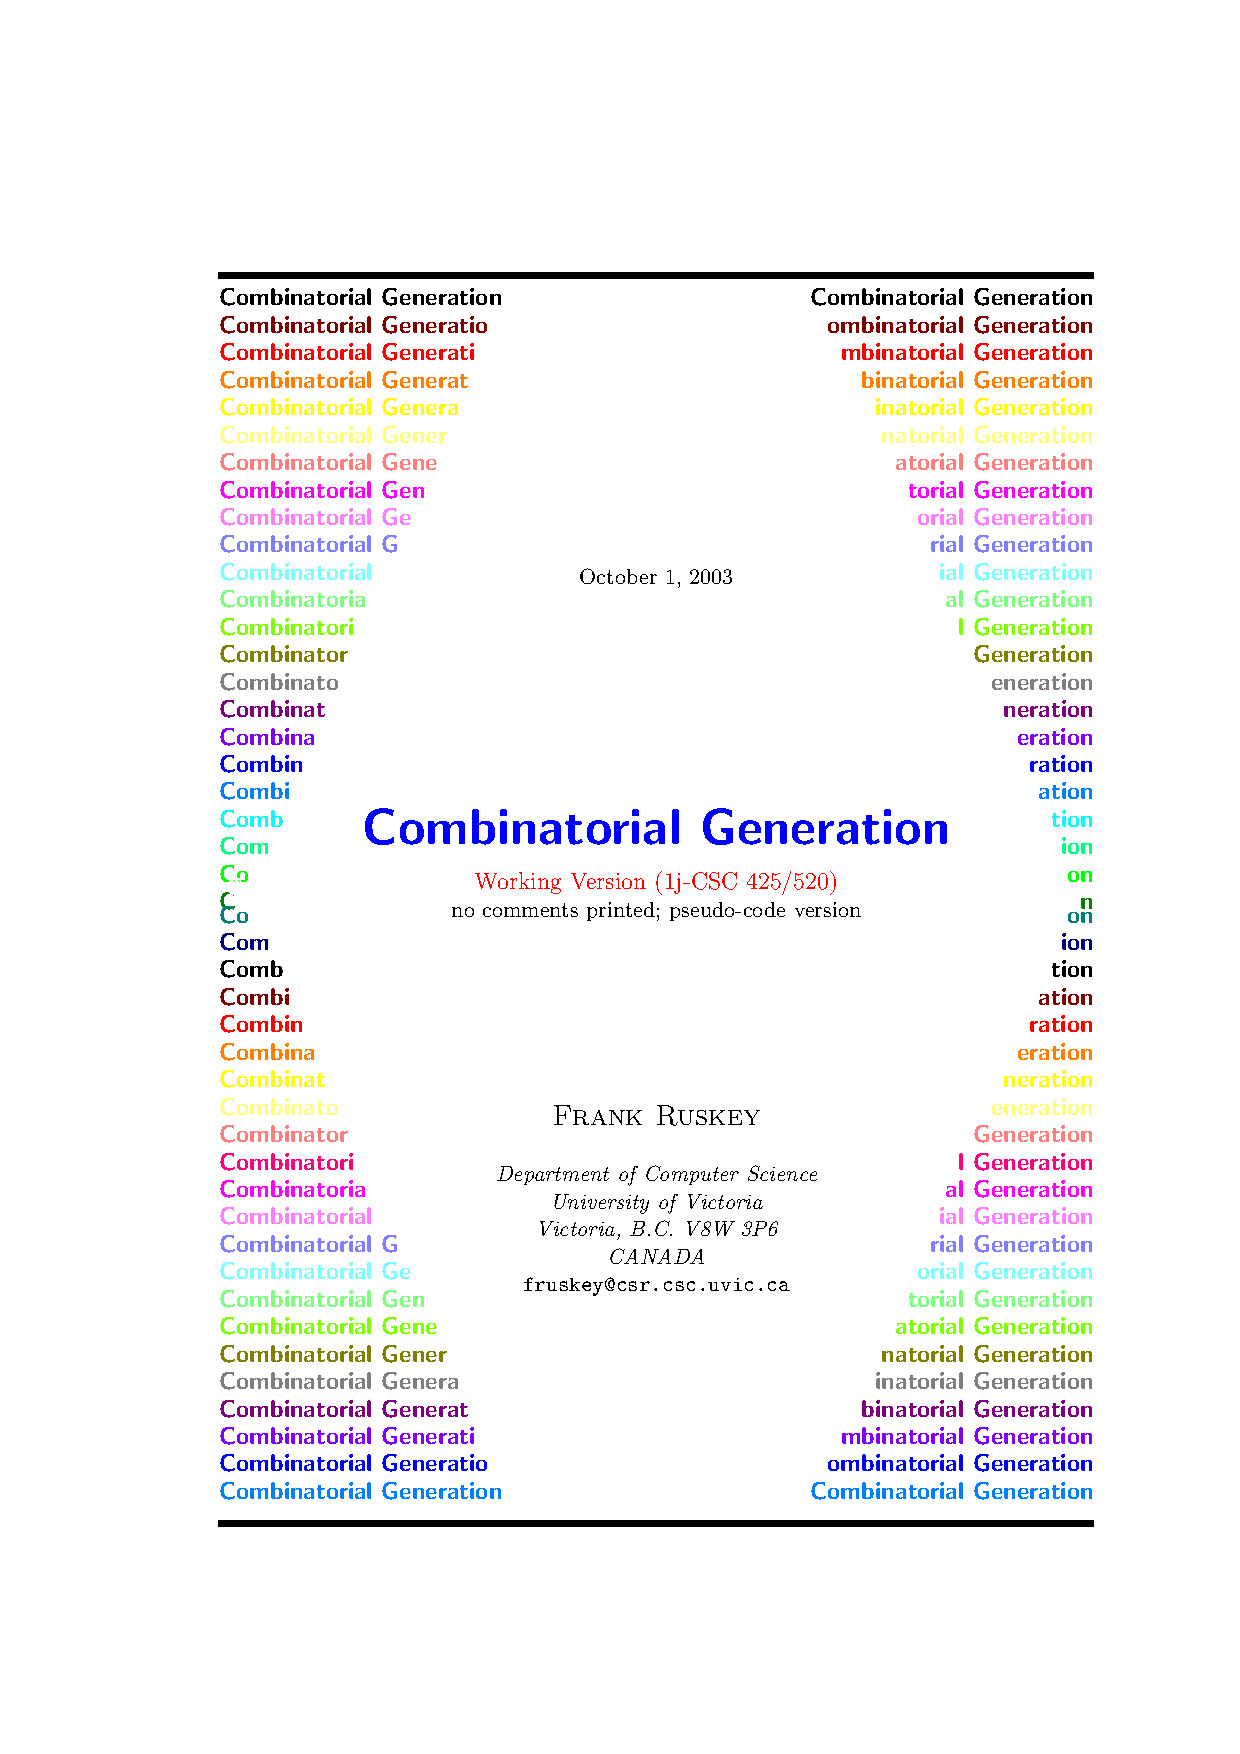
\includegraphics[width=2cm]{media/RuskeyCombGen-1.pdf}
  \end{textblock*}
\end{frame}

\begin{frame}{Generic algorithms}
  \begin{QUESTION}
    \Large
    How to avoid \textit{ad hoc} solution for each and every type of
    combinatorial objects ?
  \end{QUESTION}
  \pause\bigskip
   \begin{itemize}
   \item \textbf{basic components}
     $\Longrightarrow$ singleton, union, cartesian product, set and
     multiset, cycle\dots\pause\bigskip
   \item \textbf{combine} the basic components
     $\Longrightarrow$ combinatorial class, description grammar
   \end{itemize}
  \pause\bigskip

  \red{\Large\bf Today: Only counting !}
\end{frame}


\section{Combinatorial Classes and the Symbolic Method}

\begin{frame}{Notion of combinatorial class}
  \begin{DEFN}[Combinatorial class]
    A \emph{combinatorial class}, is a finite or denumerable set $\mC$ whose
    elements $e$ have a size (also called degree) noted $|e|$, satisfying the
    following conditions:
    \begin{itemize}
    \item the size of an element is a non-negative integer
    \item the number of elements of any given size is finite
    \end{itemize}
    \[
    \card\{\in \mC\ \mid\ |e| = n\} < \infty
    \]
  \end{DEFN}
  \bigskip

  Example:
  \begin{itemize}
  \item Binary trees where size is the number of nodes
  \end{itemize}
\end{frame}

\begin{frame}{Generating series}
  
  \begin{DEFN}
    The (ordinary) \emph{generating series} of a sequence $(a_n)_n$ 
    is the formal power series
    \begin{equation*}
      A(z) := \sum_{n=0}^{\infty} a_n z^n\,.
    \end{equation*}
    The \emph{generating series} of a combinatorial class $\mA$ is the
    generating series of the numbers $a_n := \card(\mA_n)$. Equivalently,
    \begin{equation*}
      A(z) = \sum_{\alpha\in\mA} z^{|\alpha|}\,.
    \end{equation*}
  \end{DEFN}
\end{frame}

\begin{frame}{The graded disjoint union}

  If $\mC = \mA \sqcup \mB$, the elements of $\mA$ and $\mB$ keep their
  size in the graded disjoint union:

  \[\mC_n := \mA_n \sqcup \mB_n\]

  Therefore
  \[\card\mC_n = \card\mA_n + \card\mB_n\]
  \bigskip\pause

  \begin{NOTE}
    The generating series of a disjoint union is the sum of generating
    series: \[C(z) = A(z) + B(z)\,.\]
  \end{NOTE}
\end{frame}

\begin{frame}{The graded Cartesian product}

  Idea: sizes (cost, number of memory locations,
  \dots) are added:
  \[|(a, b)|_{\mA\times\mB} := |a|_\mA + |b|_\mB\]

  If $\mC = \mA \times \mB$ then
  $\displaystyle\mC_n=\bigsqcup_{i+j=n} \mA_i \times \mB_j$
  \pause

  Cardinality:
  \[ \card\mC_n = \sum_{i+j=n} \card\mA_i \cdot \card\mB_j \]
  \[[z^n](A(z)\cdot B(z)) = \sum_{i+j=n} [z^i]A(z) \cdot [X^j]B(z)\]
  \begin{NOTE}
    The generating series of a cartesian product is the product of the
    generating series: \[C(z) = A(z) \cdot B(z)\,.\]
  \end{NOTE}
\end{frame}

\begin{frame}{A dictionary : Comb. Classes / Gen. Fun. (unlabeled case)}

  \small
  \begin{tabular}{lll}
    Neutral ($|\epsilon| = 0$)& $\mE=\{\epsilon\}$ & $E(z) = 1$\\
    Atom ($|\bullet| = 1$)& $\mZ = \{\bullet\}$ & $Z(z) = z$\\
    Disjoint Union & $\mA = \mB \sqcup \mC$ & $A(z) = B(z) + C(z)$\\
    Cartesian product & $\mA = \mB \times \mC$ & $A(z) = B(z) \cdot C(z)$\\
    Sequence & $\mA = \Seq(\mB)$ & $\displaystyle A(z) = \frac{1}{1- B(z)}$ \\
    Powerset & $\mA = \PSet(\mB)$ &
      $\displaystyle A(z) =
       \exp\left(\sum_{k=1}^{\infty} \frac{(-1)^{k-1}}{k}B(z^k)\right)$ \\
    Multiset & $\mA = \MSet(\mB)$ &
      $\displaystyle A(z) =
       \exp\left(\sum_{k=1}^{\infty} \frac{1}{k}B(z^k)\right)$ \\
    Cycle    & $\mA = \Cycle(\mB)$ &
      $\displaystyle A(z) =
       \sum_{k=1}^{\infty} \frac{\phi(k)}{k}\log\frac{1}{1-B(z^k)}$
  \end{tabular}
\end{frame}

\begin{frame}[fragile]{Example : Binary trees}

  Size = number of internal nodes

  \begin{center}
  \begin{tikzpicture}[
  inner/.style={circle,draw,thick,minimum width=3mm,inner sep=0},
  triangle/.style={isosceles triangle,draw=,thick,shape border rotate=90,
    isosceles triangle stretches=true,
    minimum height=10mm,minimum
    width=15mm,inner sep=0},
  level 1/.style={sibling distance=30mm},
]
  \node[inner] {} [child anchor=north]
    child {node[triangle] {}}
    child {node[triangle] {}};
\end{tikzpicture}
  \end{center}
  \[\BinTree = \{\epsilon\}\ \sqcup\ \BinTree\times\mZ\times\BinTree\]
  \[T(z) = 1 + T(z) \cdot z \cdot T(z) = 1 + z \cdot T(z)^2\]
  \bigskip\pause

  Solution by radicals (quadratic equation):
  \[T(z) = \frac{1 - \sqrt{1-4z}}{2z}\]
\end{frame}

\begin{frame}{Summary: Why generating series ?}

  \begin{NOTE}[The symbolic method]
    \begin{itemize}
    \item \blue{describe} combinatorial objects by \emph{grammars} using
      basic elementary constructions
    \item \blue{translate} these grammar to \emph{systems of functional
        equations} on generating series
    \item «\blue{solve}» \red{these systems} by algebraic manipulation allows
      to extract the coefficients
    \end{itemize}
  \end{NOTE}
  \bigskip
  
  Going further: \blue{asymptotic analysis} thanks to \blue{complex analysis}
\end{frame}

\section{Formalizing Formal Power Series}

\begin{frame}{What are power series ?}

  $K$ : a ring.
  \bigskip

  \begin{definition}
    The ring $K[[X]]$ of \emph{formal power series} is the set of sequences
    $(a_n)_n$, written as $\sum_n a_n X^n$ together with the natural sum, and
    product.
  \end{definition}
  More structures: derivation, integration, substitution\dots
  \pause\bigskip

  Problem: series are infinite objects
  \begin{itemize}
  \item Impossible to store one in a finite data structure
    \medskip

  \item Equality cannot be decided (MathComp requirement)
  \end{itemize}
\end{frame}

\begin{frame}{Two possible implementations}

  \begin{NOTE}
    \begin{itemize}
    \item \emph{truncated formal power series} : For a fixed $n$, we only
      know coefficients upto $x^n$ \bigskip

    \item infinite \emph{formal power series} : we store all the coefficient
      but we need \blue{infinite objects and classical axioms}
    \end{itemize}
  \end{NOTE}
  \bigskip

  Remark: this is also a problem in Computer Algebra Systems
\end{frame}


\begin{frame}[fragile]{Power series in Sagemath}

  \scriptsize
  \begin{minted}{python}
sage: F.<z> = LazyPowerSeriesRing(QQ)   # coeff. computed on demand
sage: T = 1/(1-z); T
Uninitialized lazy power series
sage: T[3]
1
sage: T
1 + z + z^2 + z^3 + O(x^4)
sage: T[5]
1
sage: T
1 + z + z^2 + z^3 + z^4 + z^5 + O(x^6)

sage: FF.<x> = PowerSeriesRing(QQ)     # truncated (to X^20 by default)
sage: T = 1/(1-x)
sage: T
1 + x + x^2 + x^3 + x^4 + x^5 + x^6 + x^7 + x^8 + x^9 +
 x^10 + x^11 + x^12 + x^13 + x^14 + x^15 + x^16 + x^17 +
 x^18 + x^19 + O(x^20)
sage: T[40]
IndexError: coefficient not known
  \end{minted}
\end{frame}

\begin{frame}[fragile]{Truncated formal power series}

  \begin{DEFN}
    The ring $K[[X]]_n$ of \emph{$n$~th-Truncated power series} is
    the quotient ring $K[X]/\langle x^n\rangle$.
  \end{DEFN}
  \bigskip\pause

  Major rewrite of the code from Cyril Cohen and Boris Djalal to adapt it to
  any ring (e.g. $\Z$) -- not just a field.  \bigskip

  Truncation = cutting a list (instead of taking the remainder in the
  Euclidian division).
\end{frame}

\begin{frame}[fragile]{Truncated formal power series}
  Definition:
  \begin{coqcode}
Variable R : ringType.
Variable n : nat.
Record truncfps := MkTfps { tfps : {poly R}; _ : size tfps <= n.+1 }.
  \end{coqcode}
  \bigskip

  Extracting coefficients:
  \begin{coqcode}
Implicit Types (p q r s : {poly R}) (f g : {tfps R n}).

Lemma coef_tfps f i : f`_i = if i <= n then f`_i else 0.
Lemma tfpsP f g : (forall i, i <= n -> f`_i = g`_i) <-> (f = g).
  \end{coqcode}

\end{frame}


\begin{frame}[fragile]{Truncated formal power series (2)}

  Polynomial truncation
  \begin{coqcode}
Fact trXn_subproof p : size (Poly (take n.+1 p)) <= n.+1.
Definition trXn p := MkTfps (trXn_subproof p).
  \end{coqcode}
  \bigskip\pause

  gives the ring structure:
  \begin{coqcode}
Lemma trXn_mul p q :
  trXn n (tfps (trXn n p) * tfps (trXn n q)) = trXn n (p * q).

Fact one_tfps_proof : size (1 : {poly R}) <= n.+1.
Definition one_tfps : {tfps R n} := Tfps_of one_tfps_proof.

Definition mul_tfps f g := trXn n (tfps f * tfps g).
\end{coqcode}
\end{frame}

\begin{frame}[fragile]{More structure on formal power series}

  Example: if $R$ is a unitary ring then $R[[X]]_n$ is too.

  \begin{coqcode}
Variable R : unitRingType.
Definition unit_tfps : pred {tfps R n} := fun f => f`_0 \in GRing.unit.
\end{coqcode}

Definition by fixed point:
\begin{coqcode}
Fixpoint inv_tfps_rec f bound m :=
  if bound is b.+1 then
    if (m <= b)%N then inv_tfps_rec f b m
    else -f`_0%N^-1 * (\sum_(i < m) f`_i.+1 * (inv_tfps_rec f b (m - i.+1)%N))
  else f`_0%N^-1.
Definition inv_tfps f : {tfps R n} :=
  if unit_tfps f then [tfps i <= n => inv_tfps_rec f i i] else f.
\end{coqcode}

\begin{coqcode}
Lemma mul_tfpsVr : {in unit_tfps, right_inverse 1 inv_tfps *%R}.
Lemma mul_tfpsrV : {in unit_tfps, left_inverse 1 inv_tfps  *%R}.
\end{coqcode}
\end{frame}

\begin{frame}[fragile]{More structure on formal power series}

  Example: formal derivative

\begin{coqcode}
Definition deriv_tfps f := [tfps j <= n.-1 => f`_j.+1 *+ j.+1].

deriv_tfps
     : {tfps R n} -> {tfps R n.-1}
\end{coqcode}

Classical formulas
\begin{coqcode}
Fact derivD_tfps f g : (f + g)^`() = f^`()%tfps + g^`()%tfps.
Theorem derivM_tfps n (f g : {tfps R n}) :
  (f * g)^`() = f^`()%tfps * (trXnt n.-1 g) + (trXnt n.-1 f) * g^`()%tfps.
\end{coqcode}
\bigskip\pause

All the formula for analysis:
\begin{itemize}
\item primitive
\item exponential, logarithm
\item composition $F(G(X))$ (needs $G_0 = 0$ no convergence).
\end{itemize}
\end{frame}

\begin{frame}{Infinite power series}

  Using the classical axiom from Mathcomp's analysis.
  \bigskip

  \begin{PROBLEM}
    One can construct them \blue{from scratch}, but one has to \red{redo all
      the work of polynomials}.
  \end{PROBLEM}
  \bigskip\bigskip\pause

  \begin{QUESTION}
    Is there a way to get infinite power series from truncated one ?
  \end{QUESTION}
  \bigskip\pause

  Limit of $K[[X]]_n$ as $n$ tends to infinity ? In what sense ?
\end{frame}

\begin{frame}[fragile]{Inverse (projective) systems}

  \begin{itemize}
  \item $I$: ordered directed set -- only need nonnegative integers.
  \item In an algebraic category (e.g. ring with ring morphisms)
  \end{itemize}
  \begin{DEFN}
    An \emph{inverse system} is given by
    \begin{itemize}
    \item \blue{Objects}: a sequence $(A_i)_{i\in I}$
    \item \blue{Bonding morphisms}: for each $i\leq j$ a morphism
      $\phi_{i,j}: A_j\mapsto A_i$ (\red{beware the inverse direction}).
    \end{itemize}
    such that for all $i\in I$, the morphism $\phi_{i,i}$ is the identity and
    \begin{itemize}
    \item \blue{Compatibility}: for all $i \leq j \leq k$, one has
      $\phi_{i,j} \circ \phi_{j,k} = \phi_{i,k}$
      \vskip-3mm
\[
\begin{tikzcd}%[row sep=4em]
  A_{i}
  & A_{j} \arrow[l,"\phi_{ij}",swap]
  & A_{k} \arrow[l,"\phi_{jk}",swap] \arrow[ll,"\phi_{ik}",bend
  right=40,swap]
\end{tikzcd}
\]
\end{itemize}
  \end{DEFN}
\end{frame}

\begin{frame}[fragile]{Inverse (projective) systems}

  \begin{DEFN}
    An \emph{inverse limit} of an inverse system, is given by
    \begin{itemize}
    \item \blue{Object}: $A$
    \item \blue{Projection morphisms}: for each $i$ a morphism
      $\mu_{i}: A\mapsto A_i$.
    \end{itemize}
      such that
    \begin{itemize}
    \item \blue{Compatibility}: for all $i \leq j$, one has
      $\phi_{i,j} \circ \mu_{j} = \phi_{i}$
    \end{itemize}
  \end{DEFN}
\[
\begin{tikzcd}%[row sep=4em]
  A_{i}
  & A_{j} \arrow[l,"\phi_{ij}",swap]
  & A_{k} \arrow[l,"\phi_{jk}",swap] \arrow[ll,"\phi_{ik}",bend
  right=40,swap]\\
  & A \arrow[ul,"\mu_{i}"] \arrow[u,"\mu_{j}",swap]
  \arrow[ur,"\mu_{k}",swap]
\end{tikzcd}
\]

\end{frame}

\begin{frame}[fragile]{Inverse limits universal property}

  \begin{THEO}
    Inverse limit \blue{do exists and are unique} (upto isomorphism) in most
    algebraic categories.
  \bigskip

  Universal property:
\[
\begin{tikzcd}
  A_{i}& & A_{j} \arrow[ll,"\phi_{ij}",swap] \\
  & A \arrow[ul,"\mu_{i}",swap] \arrow[ur,"\mu_{j}"]\\
  & Y \arrow[u,"U",swap]
  \arrow[uul,"\nu_{i}",end anchor={[xshift=0.2em]south}]
  \arrow[uur,"\nu_{j}",end anchor={[xshift=-0.2em]south},swap]
\end{tikzcd}
\]
  \end{THEO}
\end{frame}


\begin{frame}{Proof of the abstract nonsense}

  Dealing with concrete categories (Objects are Sets).
  \bigskip

  \begin{DEFN}
    A \emph{cone} of an inverse system is a sequence $c=(c_i)_{i\in I}$ where
    $x_i\in A_i$ such that \[\phi_{i,j}(c_j) = c_i\,.\]
  \end{DEFN}
  Defining
  \begin{itemize}
  \item $A$ : the set of cones
  \item $\mu_i(c) := c_i$.
  \end{itemize}
  constructs indeed an inverse limit !
\end{frame}


\begin{frame}[fragile]{Inverse systems and limits in Mathcomp}
\begin{coqcode}
Variable Obj : I -> Type.
Variable bonding : (forall i j, i <= j -> Obj j -> Obj i).
Record invsys : Type := InvSys {
      invsys_inh : I;
      invsys_id  : forall i (Hii : i <= i), (bonding Hii) =1 id;
      invsys_comp : forall i j k  (Hij : i <= j) (Hjk : j <= k),
          (bonding Hij) \o (bonding Hjk) =1 (bonding (le_trans Hij Hjk));
  }.
(* The Mixin formalizes the universal property *)
Record mixin_of (TLim : Type) := Mixin {
  invlim_proj : forall i, TLim -> Obj i;
  invlim_ind  : forall (T : Type) (f : forall i, T -> Obj i),
      (cone Sys f) -> T -> TLim;
  _ : cone Sys invlim_proj;
  _ : forall T (f : forall i, T -> Obj i) (Hcone : cone Sys f),
      forall i, invlim_proj i \o invlim_ind Hcone =1 f i;
  _ : forall T (f : forall i, T -> Obj i) (Hcone : cone Sys f),
      forall (ind : T -> TLim),
        (forall i, invlim_proj i \o ind =1 f i) ->
        ind =1 invlim_ind Hcone
  }.
\end{coqcode}
\end{frame}

\begin{frame}[fragile]{Back to power series}

\begin{coqcode}
Definition fps_bond := fun (i j : nat) of (i <= j)%O => @trXnt R j i.

Record fpseries := FPSeries { seriesfun : nat -> R }.
Definition fpsproj n (f : {fps R}) : {tfps R n} := [tfps i <= n => f``_i].
Lemma fpsprojP : cone fps_invsys fpsproj.

Notation "''pi_' i" := (fpsproj i).
Lemma fpsprojE x y : (forall i : nat, 'pi_i x = 'pi_i y) -> x = y.

Canonical fps_invlimType := Eval hnf in InvLimType {fps R} fps_invlimMixin.
\end{coqcode}
Now algebraic structures are for free:
\begin{coqcode}
Canonical fps_zmodType :=
  Eval hnf in ZmodType {fps R} [zmodMixin of {fps R} by <-].
Canonical fps_ringType :=
  Eval hnf in RingType {fps R} [ringMixin of {fps R} by <-].
[...]
\end{coqcode}
\end{frame}

\begin{frame}[fragile]{Back to power series}

One can reuse everything from truncated power series !
\bigskip

Example: derivative of a product:
\begin{coqcode}
Theorem derivM_tfps n (f g : {tfps R n}) :
  (f * g)^`() = f^`()%tfps * (trXnt n.-1 g) + (trXnt n.-1 f) * g^`()%tfps.

Theorem derivM_fps (f g : {fps R}) :
  (f * g)^`()%fps = f^`()%fps * g + f * g^`()%fps.
Proof.
apply invlimE => i.
rewrite !(proj_simpl, proj_deriv_fps) derivM_tfps /=.
by rewrite -!fps_bondE !ilprojE.
Qed.
\end{coqcode}
\end{frame}

\section{The example of Catalan numbers}

\begin{frame}[fragile]{Back to Catalan numbers}

  \begin{THEO}
    Suppose that $(C_i)_{i\in\N}$ verifies
    \[ C_0 = 1 \qandq C_n=\sum_{k=0}^{n-1}C_k C_{n-1-k}\,,\]
    then
    \[\displaystyle T_n=\frac{1}{n+1}\binom{2n}{2}\]
  \end{THEO}

\begin{coqcode}
forall C : nat -> nat,
       C 0 = 1 ->
       (forall n : nat, C n.+1 = \sum_(i < n.+1) C i * C (n - i)) ->
       forall i : nat, C i = 'C(i.*2, i) %/ i.+1
\end{coqcode}
\end{frame}

\begin{frame}[fragile]{Proofs in mathcomp}
  \[2\times 3 + 1 = 7 \text{ proofs !}\]
  \begin{itemize}
  \item Truncated or infinite power series
  \end{itemize}

\begin{coqcode}
Definition FC : {fps Rat} := \fps (C i)%:R .X^i.
Proposition FC_algebraic_eq : FC = 1 + ''X * FC ^+ 2.

Definition FC : {tfps Rat n} := [tfps i => (C i)%:R].
Proposition FC_algebraic_eq : FC = 1 + \X * FC ^+ 2.
\end{coqcode}
\bigskip

3 methods to extract the coefficients:
\begin{itemize}
\item generalized Newton binomial formula
\item Lagrange inversion formula
\item holonomic computation
\end{itemize}
\bigskip

+ 1 bijective proof
\end{frame}

\begin{frame}[fragile]{Generalized Newton binomial formula}

  \[F(X) = \frac{1 - \sqrt{1-4X}}{2X}\]

  \begin{THEO}
    For any $\alpha$ (non necessarily integer):
    \[
      (1+X)^\alpha =
      \sum_n \frac{\alpha(\alpha -1)\dots(\alpha - m + 1)}{m!} X^n
    \]
  \end{THEO}

\begin{coqcode}
Theorem coef_expr1cX c a m :
  ((1 + c *: ''X) ^^ a)%fps``_m =
  c ^+ m * \prod_(i < m) (a - i%:R) / m`!%:R :> R.
\end{coqcode}
\end{frame}

\begin{frame}{General methods ?}

  \begin{PROBLEM}
    Newton's only works for equation which are solvable by radicals.
  \end{PROBLEM}
  \bigskip

  More general solutions:
  \begin{itemize}
  \item Lagrange inversion
  \item Holonomic computation
  \end{itemize}
\end{frame}

\begin{frame}[fragile]{Lagrange formula}
  Fact: $\{\text{series starting with } X\}$ is a group for $\circ$ (neutral $X$).
  \begin{PROP}[Lagrange Inversion]
    $F(X)=X + \dots$ has a \emph{unique inverse} $F^*$ (Lagrange inverse):
    \[ F(F^*(X)) = F^*(F(X)) = X\,.\]

    Writing $F=\frac{X}{G}$ fixed point version
    $F^*(X) = X\cdot G(F^*(X))\,.$

    Its coefficient are given by
    $\displaystyle[X^{i+1}](F^*) = \frac{[X^{i}](G^{i+1})}{i+1}\,.$
  \end{PROP}
  For catalan: $G(X) = (1 + X)^2$
  \begin{coqcode}
Proposition FC_fixpoint_eq : FC - 1 = lagrfix ((1 + ''X) ^+ 2).
  \end{coqcode}
\end{frame}

\begin{frame}[fragile]{Holonomic computation}
  \begin{itemize}
  \item $F$ is \emph{rational} if $F = \frac{N}{P}$ with $N, P$ polynomials.
  \item $F$ is \emph{algebraic} if there exists polynomials
    $(P_0, \dots, P_d)$ s.t.
    \[P_0 + P_1 F + P_2 F^2 + \dots P_d F^d = 0\,.\]

  \item $F$ is \emph{holonomic} if there exists polynomials
    $(P_c, P_0, \dots, P_d)$ s.t.
    \[P_C + P_0 F + P_1 F' + P_2 F'' + \dots P_d F^{(d)} = 0\,.\]
  \end{itemize}
  \begin{theorem}
    \begin{center}
      rational $\quad\to\quad$ algebraic $\quad\to\quad$ holonomic.
    \end{center}
  \end{theorem}
\end{frame}

\begin{frame}[fragile]{Catalan from holonomic computation}
  \[F = 1 + X \cdot F ^2\]
  gives
  \[(1 - X^2) F + (1 - X^4) X F' = 1\,.\]
  \begin{coqcode}
Proposition FC_differential_eq n :     (* truncated series version *)
   (1 - \X *+ 2) * (FC n.+1) + (1 - \X *+ 4) * tmulX (FC n.+1)^`() = 1.

Proposition FC_differential_eq :       (* infinite series version *)
  (1 - ''X *+ 2) * FC + (1 - ''X *+ 4) * ''X * FC^`() = 1.
\end{coqcode}
\bigskip

  Extracting the coefficients gives the simplest possible recurrence:
  \[(n+2) C_{n+1} = (4n + 2) C_{n}\,.\]
\end{frame}

\section{Conclusion}

\begin{frame}{Conclusion}

  \begin{itemize}
  \item Once we have the formalization of power series, using them is quite
    simple (300 lines for the three proofs)
  \item I strongly regret I didn't had them for Littlewood-Richardson !
  \item Automation (eg: \texttt{ring} tactic) should make it even shorter;
  \item Much shorter that the bijective proofs (500 lines);
  \item Using truncated power series makes the proof only slightly longer (to
    deal with the degree bound), but the statement more complicated (degree
    bound, 2 different multiplications by X, keeping or adding one to the
    degree).
  \item Work in progress on limits (need help with
    Canonical / Mixin / HierarchyBuilder).
  \item Everything I presented here could be entirely automatized thanks to
    computer algebra (see e.g. \texttt{combstruct} Maple\textcopyright).
  \end{itemize}
\end{frame}

\end{document}

%%% Local Variables:
%%% mode: latex
%%% TeX-master: t
%%% End:
